\chapter{Extendiendo el borrow checker}

El borrow checker es un componente del compilador de Rust que verifica que el código fuente cumpla con las reglas de Ownership y Borrowing del lenguaje. En otras palabras, el borrow checker analiza el código para asegurarse de que no haya más de una referencia mutable a un mismo valor al mismo tiempo, que las referencias no sobrevivan al valor al que hacen referencia y que no haya referencias inválidas. Si el borrow checker encuentra algún problema, el compilador genera un error de compilación para ayudar al programador a corregir el código. El borrow checker es una parte esencial de Rust que ayuda a prevenir errores comunes de programación, como la corrupción de memoria y los errores de concurrencia.

Nuestro objetivo es extender la funcionalidad del mismo incorporando nuevos análisis estáticos como Stacked Borrows\cite{stackedborrows} para poder tratar de capturar nuevos errores enfocándonos en los problemas de aliasing, y además, poder realizar estas detecciones en código unsafe donde el sistema de borrow-checking se encuentra deshabilitado y por lo tanto se pierden estas ventajas de seguridad en el manejo de memoria intrínsecas al lenguaje.

\section{Etapas del proceso de compilación}

El compilador de Rust según \cite{rustcdevelopment} se diferencia del resto, ya que hace procesos que otros no realizan (borrow-checking) y también toma algunas decisiones no convencionales. El proceso de compilación de un programa comienza al invocar el comando \textbf{rustc} junto al código fuente de un programa y los parámetros. El módulo \textit{rustc\_driver} se encarga de captar los argumentos y definir la configuración que se utilizará en el resto del procedimiento.

Una vez que el compilador captó el código, los módulos \textit{rustc\_lexer} y \textit{rustc\_parse} se encargan de analizarlo y generar el AST (árbol de sintaxis abstracta). En esta primera etapa también se expanden las macros, se resuelven los nombres, se chequea la sintaxis del programa y sé valida que el AST sea correcto.

\begin{wrapfigure}{r}{0.25\textwidth}
    \caption{Compiler pipeline}
    \centering
    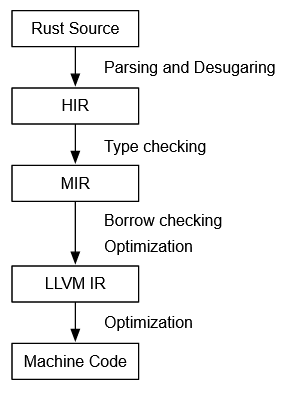
\includegraphics[width=0.3\textwidth]{compiler-flow}
\end{wrapfigure}

Teniendo este árbol, se proceden a generar las representaciones intermedias. La primera en construirse es el HIR (High-Level Intermediate Representation) que es una versión más amigable para el compilador del AST. Durante este proceso se realiza la inferencia de tipos, la resolución de las traits y principalmente el chequeo de tipos, donde se convierten los tipos encontrados en el HIR por representaciones internas usadas por el compilador. Estas son usadas para aumentar la seguridad, correctitud y coherencia de los tipos utilizados en el programa.

La siguiente parte es la construcción del MIR (Mid-Level Intermediate Representation) a partir del HIR. Aquí es donde se hacen gran parte de las optimizaciones del código, junto al pattern-matching y chequeos de exhaustividad. Además, el MIR es donde se realiza el \text{borrow-checking} y otros chequeos importantes basados en el flujo de datos. Debido a que es una representación de alto nivel y genérica es aquí donde se realizan la mayoría de análisis del compilador, y nosotros tomaremos en cuenta esto para añadir nuestros propios algoritmos y análisis.

A continuación se realiza lo que es conocido por la generación de código o \textit{codegen}, que consiste en transformar las representaciones de alto nivel a un binario executable. \textbf{Rustc} utiliza \textbf{LLVM} para esto. Se comienza convirtiendo el MIR en LLVM IR (LLVM Intermediate Representation) para luego pasárselo a LLVM, el cual realiza más optimizaciones, y emitir el código de máquina. Este es básicamente código assembler con algunos tipos y anotaciones añadidos. Los diferentes binarios/bibliotecas luego son unidos (linked) para crear el binario final.

\section{Análisis estáticos}

El análisis estático de programas es una técnica que se utiliza para examinar el código fuente de un programa sin necesidad de ejecutarlo, con el objetivo de encontrar errores o posibles problemas. Algunas de las ventajas del análisis estático incluyen la detección temprana de errores, la identificación de vulnerabilidades de seguridad y la mejora de la eficiencia del código. Las herramientas de análisis estático se utilizan comúnmente en muchos lenguajes de programación, incluyendo Rust, y pueden detectar una amplia gama de errores de programación, como errores de sintaxis, errores de tipo, fugas de memoria y problemas de concurrencia, entre otros.

En esta sección describiremos con detalle los diferentes conceptos y particularidades de los análisis estáticos que implementaremos en nuestra herramienta como lo son Stacked Borrows y análisis de alias points-to, y además nos expandiremos en la definición del MIR y su amplia utilidad como base para el desarrollo de nuestro programa. 

\subsection{MIR}

\cite{rustcdevelopment} dice el MIR que es una forma simplificada de Rust el compilador utiliza principalmente para comprobaciones de seguridad flow-sensitive, como por ejemplo el borrow checker. Está definido en el módulo \textbf{rust\_middle::mir}, se basa en un CFG (Control-Flow Graph o Grafo de Control de Flujo) y todos los tipos son explícitos.

El CFG es un término común en el ámbito de los compiladores, ya que permite representar un programa exponiendo de manera clara el flujo del mismo. El CFG del MIR está estructurado como un conjunto de bloques básicos conectados por aristas. Estos bloques básicos están conformados por un conjunto de \textit{statements} que se ejecutarían juntos y de manera secuencial y completa. Al final se encuentra un \textit{terminator} cuya función es referenciar y conectar bloques básicos. La construcción de un CFG es generalmente el primer paso de la mayoría de los algoritmos de análisis flow-sensitive, y el MIR está estructurado de esta manera para facilitar estos análisis.

Otros conceptos claves del MIR son:
\begin{itemize}
    \item \textbf{Locals}: Lugar de la memoria alojado (conceptualmente) en el stack. Se representan con un guion bajo seguido de un número, por ejemplo \_1. El lugar \_0 está reservado para la dirección de retorno de la función.
    \item \textbf{Places}: Expresiones que identifican un lugar en la memoria.
    \item \textbf{Rvalues}: Expresiones que producen un valor. Su nombre proviene del hecho de que están del lado derecho de una asignación.
    \begin{itemize}
        \item \textbf{Operands}: Son los argumentos de un rvalue, que pueden ser constantes o Places
    \end{itemize}
\end{itemize}

Mediante el uso de las versiones nightly del compilador, que añaden la posibilidad de importar módulos críticos e imperativos para los análisis estáticos que queremos realizar, es posible acceder y utilizar las distintas representaciones intermedias de un código fuente.

Podemos apreciar la transformación a MIR mediante un ejemplo. El siguiente programa básico
\begin{lstlisting}[language=Rust]
    fn main() {
        let mut x = 5;
        x = x + 10;
    }
\end{lstlisting}
tiene una representación en MIR de la siguiente forma:
\begin{lstlisting}[language=Rust]
    // WARNING: This output format is intended for human consumers only
    // and is subject to change without notice. Knock yourself out.
    fn main() -> () {
        let mut _0: ();            // return place in scope 0 at ./examples/simple_sum.rs:1:11: 1:11
        let mut _1: i32;           // in scope 0 at ./examples/simple_sum.rs:2:9: 2:14
        scope 1 {
            debug x => _1;                   // in scope 1 at ./examples/simple_sum.rs:2:9: 2:14
        }

        bb0: {
            _1 = const 5_i32;      // scope 0 at ./examples/simple_sum.rs:2:17: 2:18
            _1 = const 15_i32;     // scope 1 at ./examples/simple_sum.rs:3:5: 3:15
            return;                // scope 0 at ./examples/simple_sum.rs:4:2: 4:2
        }
    }
\end{lstlisting}

Este ejemplo, como indica el comentario arriba, muestra el MIR para que sea más sencillo de leer por las personas. Podemos apreciar como se crea la función main, se realizan las declaraciones de las variables en la parte superior y luego procede a definirse los bloques básicos. En este caso, el bloque bb0 es el único que se construyo y contiene dos statements y un terminator. Debido a las optimizaciones del compilador (propagación de constantes), los statements son solo asignaciones directas sin la necesidad de hacer una suma como en el programa fuente. El terminator en este caso es la llamada a return.

Para extender el borrow checker, se realiza una interpretación abstracta del MIR aplicando los análisis estáticos necesarios y recopilando la información.

\subsection{Stacked borrows}

Stacked Borrows \cite{stackedborrows} propone una semántica operacional para los accesos de memoria en Rust que refuerza. Stacked borrows define una disciplina de aliasing y declara que cualquier programa que la viole contendrá comportamiento no definido, lo que significa que el compilador puede descartarlos a la hora de realizar optimizaciones. Esto lo realiza introduciendo condiciones claramente definidas en las cuales un programa Rust no se comporta debidamente debido a un error de aliasing. La idea es definir una versión dinámica del \textit{borrow-checker} que Rust ya utiliza para comprobar que los accesos se hagan de acuerdo a la política de aliasing.

El borrow checker en particular comprueba que las referencias que puedan superponerse, se utilicen de una manera bien anidada. Stacked Borrows modela esta disciplina mediante un análisis haciendo uso de una pila por locación: se detecta cuando las referencias no son utilizadas que sigan una disciplina last\_in, first\_out (LIFO) en el sentido de orden de uso (el último borrow debe dejar de usarse primero), y se marca a esos programas como erróneos. Basados en eso, se extiende Stacked Borrows para las reglas de los punteros planos (que son ignorados por el borrow-checker) con el objetivo de ser lo más libres posibles sin interferir con las propiedades principales de un "fragmento seguro" del análisis que realizan.

La idea principal detrás de Stacked Borrows es tomar el análisis estático que realiza el borrow checker, el cual utiliza lifetimes, y transformarlo en un análisis dinámico el cual no haga uso de lifetimes. De esta manera, se puede lograr que inclusive aquellos programas que contengan unsafe deban satisfacer esta comprobación. Los programas Safe deberían trivialmente satisfacer el nuevo chequeo, ya que este es estrictamente más libre que el anterior.

De manera simplificada, la versión dinámica del borrow checker debería asegurar que:
\begin{enumerate}
    \item Una referencia y todas las referencias derivadas de esta puedan ser usadas solamente durante su lifetime, y
    \item El referente no es utilizado hasta que el lifetime del préstamo haya expirado.
\end{enumerate}

Consideremos el ejemplo brindado por \cite{stackedborrows}:
\begin{lstlisting}[language=Rust]
1 let mut local = 0;
2 let x = & mut local ;
3 let y = & mut *x;   // Reborrow x to y.
4 *x = 1;             // Use x again.
5 *y = 2;             // Error ! y used after x got used
\end{lstlisting}

Este programa viola el principio de pila debido a un uso de la referencia \textit{y} que ocurre en la línea 5 después del siguiente uso del referente \textit{x} en la línea 4, y por lo tanto este programa es rechazado por el borrow-checker. Si observamos el patrón de uso, podemos observar que ``XYXY'' es una violación a la idea de anidación. Para que el programa sea conforme con la política de la pila, debería tener los accesos anidados de la manera ``XYYX''.

Para llevar esta idea a cabo, Stacked Borrows define un modelo operacional. Primero se debe ser capaz de distinguir las referencias que apuntan a un mismo lugar de la memoria; por eso se asume que todas las referencias son marcadas con un ID único cuando son creadas, y este se preserva a medida que la referencia es copiada. Luego, en memoria se debe almacenar una pila que almacenará los IDs de las referencias junto a información para distinguir el tipo de item (Unique, SharedReadOnly o SharedReadWrite) que es.

Las principales reglas del modelo \label{stackedrules} son las siguientes:
\begin{itemize}
    \item (new-mutable-ref) Cada vez que una nueva referencia mutable es creada (\&mut expr) de algún valor referente existente, primero que nada se considera \textit{uso} de ese referente. Luego se elige un ID nuevo para la referencia, y se la coloca junto a su tipo (Unique) en el tope de la pila.
    \item (new-mutable-raw) Cada vez que una variable mutable plana (raw pointer) es creada mediante un casteo (expr as \*mut T) a partir de una referencia mutable (\&mut T) con el valor de algún referente, primero es considerada un uso de esa referencia mutable. Luego se añade la referencia del tipo SharedReadWrite al tope de la pila.
    \item (new-shared-ref) Cada vez que una nueva referencia compartida es creada (\&expr) a partir de un valor existente de un referente, primero es considerado un \textit{acceso de lectura} del valor. Luego se elige un ID nuevo para la referencia, y se la coloca junto a su tipo SharedReadOnly en el tope de la pila.
    \item (uso) Cada vez que un referente X es utilizado, un item con el ID X debe estar en la pila. Si existen otros items por encima de este, hay que removerlos, de tal manera que X quede en el tope de la pila. En el caso de que la pila no contenga ningún item Unique con el mismo ID del referente usado, o un valor SharedReadOnly o SharedReadWrite, entonces el programa tiene comportamiento no deseado.
    \item (lectura) Cada vez que una referencia X es leída, un item con el ID X debe encontrarse en la pila. Se remueven los elementos del tope de la pila hasta que todos los items por encima de X son SharedReadOnly. Si no existe ningún item con ID X en la pila, el programa viola el modelo planteado.
\end{itemize}

Existen ciertas extensiones y optimizaciones que pueden realizarse a este modelo, sin embargo estas son las reglas que consideramos mínimas para detectar errores de aliasing en la mayor parte de programas y son las que implementaremos en la herramienta.

Stacked borrows fue definido formalmente y está verificado utilizando Coq. Además, como hemos mencionado el intérprete MIRI \cite{miri} dentro de las variedades de chequeos que realiza, posee una implementación bastante robusta del modelo de Stacked Borrows donde se pueden realizar tests para comprobar su utilidad.

\subsection{Análisis points-to}

Existen un gran número de estudios y algoritmos realizados para el análisis del flujo de datos en los programas, y en especial para computar la información points-to. \cite{fastaliasinganalisis} establece que para realizar análisis en un programa que involucra punteros, es necesario tener información (segura) acerca de a donde apunta cada puntero. En general, mientras más precisa se tenga la información de a donde apunta (points-to), más preciso van a ser los resultados obtenidos. Los análisis de flujo de datos como propagación de constantes, variables vivas, comprobaciones de alcance, etc. necesitan saber a donde una variable podría estar apuntando en cada declaración y operación.

\cite{interprocedural} define que un Alias se produce cuando existe más de un camino de acceso a un lugar en la memoria. Un camino de acceso es un identificador que apunta a un lugar específico en la memoria, estos pueden ser punteros, expresiones conformadas por variables, etc. Dos caminos son must-alias si en una declaración S, si refieren a la misma locación en memoria en todas las instancias de ejecución de S. Dos caminos son may-alias en S si refieren a la misma locación en memoria en alguna de las ejecuciones de S, es decir, may-alias establece que pueden ser alias, pero no lo asegura. La computación de may-aliases incluye los must-aliases como subconjunto. Los algoritmos a utilizar realizaran el cálculo de los may-aliases y por el motivo anterior solamente se los mencionaran como alias.

\cite{pointeranalysis} define dos tipos comunes de análisis de punteros, que son análisis de alias y de points-to.
El análisis de alias computa un conjunto S que contenga los pares de variables (p, q) donde p y q pueden (o deben) apuntar a un mismo lugar en memoria. En cambio, el análisis points-to computa las relaciones apunta-a(p, x) donde p puede (o debe) apuntar a la locación de memoria de la variable x. Si bien ambos tienen el mismo objetivo, los métodos y algoritmos difieren. Nosotros utilizaremos un análisis points-to basado en la idea originalmente propuesta por Andersen, que es una de las más reconocidas y utilizadas para este propósito.

El análisis points-to de Andersen es interprocedural, y no tiene en cuenta el contexto o flujo. Esto quiere decir que no tiene en cuenta el orden de las declaraciones del programa, y esto se realiza para mejorar el rendimiento, ya que estos tipos de estudios pueden ser muy costosos en práctica. Sin embargo, para mejorar la precisión y debido a que el MIR es generado de manera secuencial no haremos uso de esta característica.

Para realizar este análisis, creamos un grafo dirigido para la representación de los aliases. Creamos un nodo para cada variable del programa, y haciendo una lectura secuencial de las declaraciones unimos utilizando aristas dirigidas cada vez que una variable X referencia a un valor apuntado por otra variable Y. De esta manera obtenemos todos los pares points-to(X, Y) donde X apunta a Y, y se ve reflejado en el grafo.

Este comportamiento lo podemos apreciar en el ejemplo brindado por \cite{pointeranalysis}, observando el pseudo-programa y el grafo de Andersen construido.

\begin{figure}%
    \centering
    \subfloat[\centering Pseudocodigo]{{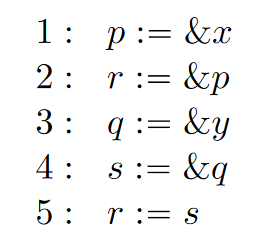
\includegraphics[width=4cm,height=5cm,keepaspectratio]{Andersen_pseudoprograma} }}%
    \qquad
    \subfloat[\centering Grafo]{{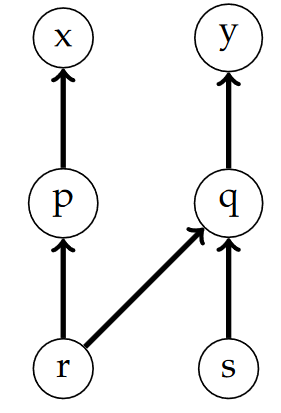
\includegraphics[width=4cm,height=5cm,keepaspectratio]{Andersen_grafo} }}%
    \caption{Creación de grafo points-to}%
\end{figure}

Una vez obtenido el grafo de points-to es posible saber cuáles variables son alias. Aquellos que nodos que tengan más de una arista entrante indican que existe más de un camino para acceder al valor ubicado en ese lugar de la memoria, y por lo tanto, se produce alias. Además, si utilizamos estos datos en conjunto la información obtenida de Stacked Borrows simulando los lifetimes de las variables, podemos añadir precisión al análisis. Esto se debe a que al realizar points-to sabemos que puede ser alias, pero no es correspondiente asegurarlo. Sin embargo, gracias a Stacked Borrows podemos saber si algunas de las referencias involucradas en el alias dejaron de utilizarse y por lo tanto, indicar una mayor posibilidad de asegurar o descartar el problema de aliasing.

Si bien este método es considerado interprocedural, es necesario tener en cuenta los aspectos mencionados por \cite{interprocedural}. Para que un análisis de flujo de datos sea interprocedural, se debe hacer uso del PCG (Program Call Graph), que es un multi-grafo en el cual cada procedimiento o función se representa como un único nodo y una arista (f, g) representa una potencial llamada a la función g desde el procedimiento f.
Si bien en el HIR es más simple obtener y navegar el PCG que se describe, se añadiría una complejidad extra al manejar ambas representaciones intermedias simultáneamente. Por eso, para reemplazar el uso del PCG se utilizan los \textit{terminator} del MIR. Estos nos brindan toda la información necesaria de las diferentes llamadas a procedimientos externos, y nos permiten mediante el estudio de los argumentos actuales y formales asociar las variables y sus lugares compartidos en la memoria entre funciones. De esta manera además ganamos eficiencia y precisión, ya que solamente tenemos en cuenta las llamadas a funciones que únicamente están relacionadas con el procedimiento que queremos analizar y que realmente sean utilizadas.

\section{Otros análisis}

Además de los análisis anteriormente mencionados, es posible realizar muchos más gracias a la gran cantidad de información presente en el MIR sin realizar grandes cambios a la estructura del proyecto. Nosotros consideramos agregar un estudio de los casts realizados de manera unsafe, en especial nos centramos en encontrar los errores que puedan surgir de hacer transformaciones de un tipo que contenga una representación de X cantidad de bits, a una que posea una cantidad diferente.

Debido a que el borrow checker está desactivado durante la creación de raw pointers, es posible hacer casts de tipos las restricciones convencionales. Por ejemplo, se podría intentar trasformar un flotante f32 que necesita mínimo de 32 bits, utilizando un puntero plano, a un entero u16 que necesita mínimo de 16 bits. Esto claramente es un problema, ya que si intentamos utilizar este entero es muy probable que se produzca comportamiento no deseado, ya que estamos quitándole arbitrariamente la mitad de la información del tipo original sin hacer ningún chequeo de sí el resultado sea correcto.

Para realizar esta comprobación simplemente recorremos el normalmente MIR hasta encontrar una sentencia de Cast. Una vez que se encuentre, observamos las variables involucradas y obtenemos la información de sus respectivas representaciones. Con estos datos, procedemos a comparar estas representaciones con base en la cantidad de bytes que posean, y si encontramos que no poseen la misma cantidad y que se está intentando transformar una representación de mayor cantidad de datos a de menor cantidad, se procede a informar de la situación. De esta manera, el programador podrá ver el aviso y tomar los recaudos necesarios para asegurarse de que este problema no rompa la política de seguridad de Rust.